% Created by tikzDevice version 0.12.6 on 2026-10-26 12:43:26
% !TEX encoding = UTF-8 Unicode
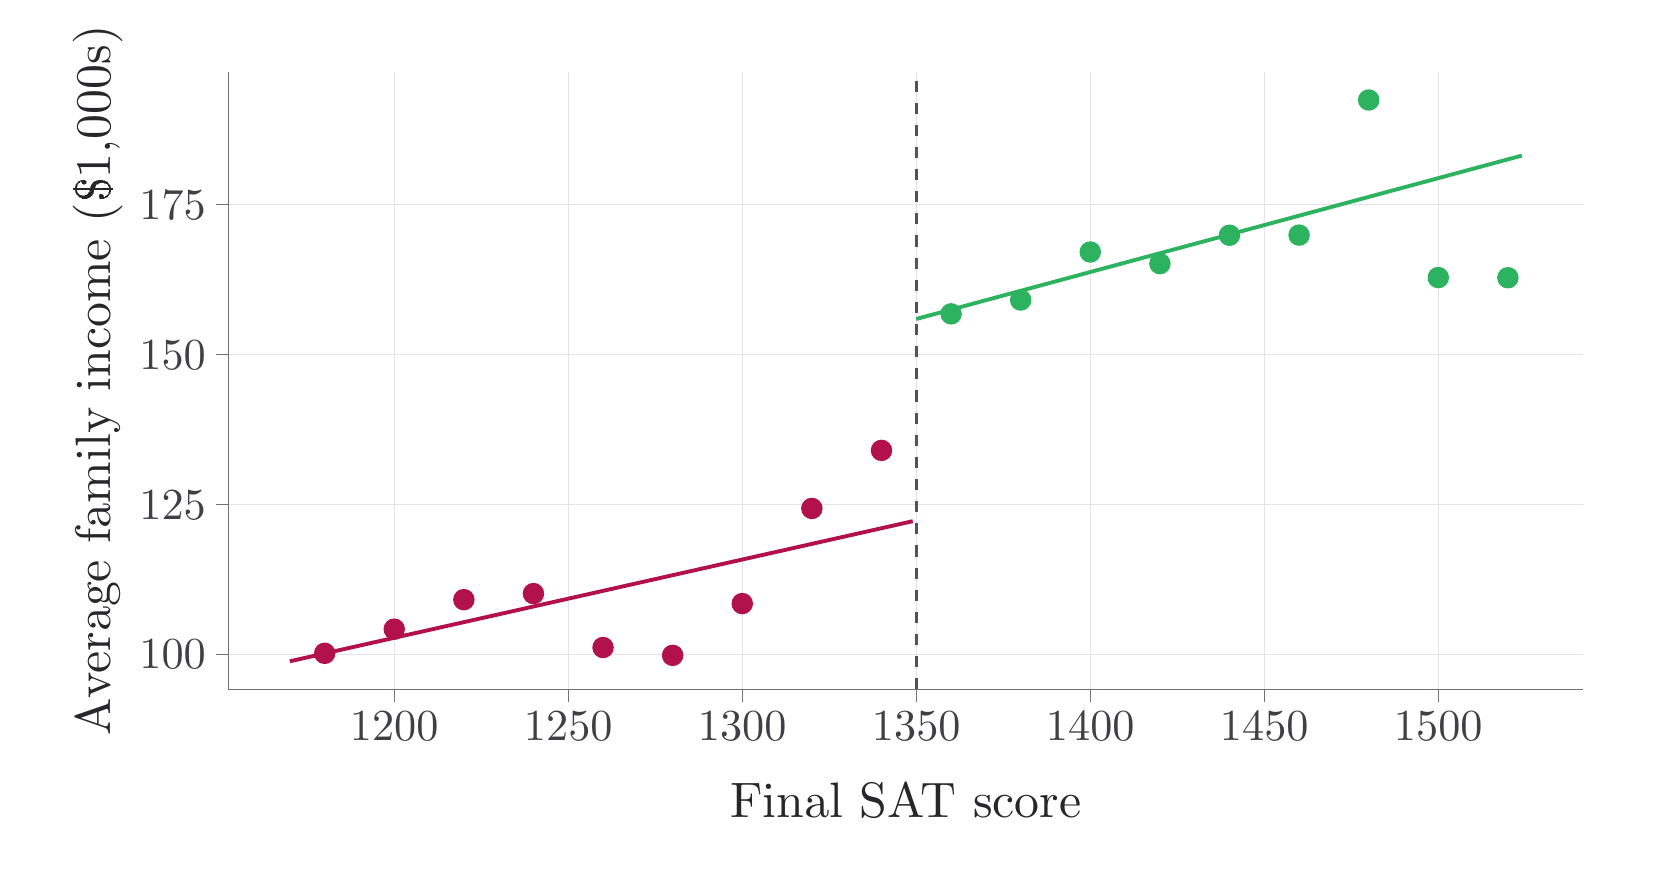
\begin{tikzpicture}[x=1pt,y=1pt]
\definecolor{fillColor}{RGB}{255,255,255}
\path[use as bounding box,fill=fillColor] (0,0) rectangle (578.16,303.53);
\begin{scope}
\path[clip] (  0.00,  0.00) rectangle (578.16,303.53);
\definecolor{drawColor}{RGB}{255,255,255}

\path[draw=drawColor,line width= 0.9pt,line join=round,line cap=round,fill=fillColor] (  0.00,  0.00) rectangle (578.16,303.53);
\end{scope}
\begin{scope}
\path[clip] ( 72.48, 64.43) rectangle (562.16,287.53);
\definecolor{drawColor}{RGB}{255,255,255}
\definecolor{fillColor}{RGB}{255,255,255}

\path[draw=drawColor,line width= 0.9pt,line join=round,line cap=round,fill=fillColor] ( 72.48, 64.43) rectangle (562.16,287.53);
\definecolor{drawColor}{RGB}{228,228,231}

\path[draw=drawColor,line width= 0.4pt,line join=round] ( 72.48, 77.06) --
	(562.16, 77.06);

\path[draw=drawColor,line width= 0.4pt,line join=round] ( 72.48,131.22) --
	(562.16,131.22);

\path[draw=drawColor,line width= 0.4pt,line join=round] ( 72.48,185.39) --
	(562.16,185.39);

\path[draw=drawColor,line width= 0.4pt,line join=round] ( 72.48,239.56) --
	(562.16,239.56);

\path[draw=drawColor,line width= 0.4pt,line join=round] (132.46, 64.43) --
	(132.46,287.53);

\path[draw=drawColor,line width= 0.4pt,line join=round] (195.34, 64.43) --
	(195.34,287.53);

\path[draw=drawColor,line width= 0.4pt,line join=round] (258.21, 64.43) --
	(258.21,287.53);

\path[draw=drawColor,line width= 0.4pt,line join=round] (321.09, 64.43) --
	(321.09,287.53);

\path[draw=drawColor,line width= 0.4pt,line join=round] (383.97, 64.43) --
	(383.97,287.53);

\path[draw=drawColor,line width= 0.4pt,line join=round] (446.84, 64.43) --
	(446.84,287.53);

\path[draw=drawColor,line width= 0.4pt,line join=round] (509.72, 64.43) --
	(509.72,287.53);
\definecolor{drawColor}{RGB}{82,82,91}

\path[draw=drawColor,line width= 1.1pt,dash pattern=on 4pt off 4pt ,line join=round] (321.09, 64.43) -- (321.09,287.53);
\definecolor{drawColor}{RGB}{179,17,75}
\definecolor{fillColor}{RGB}{179,17,75}

\path[draw=drawColor,line width= 0.6pt,line join=round,line cap=round,fill=fillColor] (132.46, 86.17) circle (  3.58);

\path[draw=drawColor,line width= 0.6pt,line join=round,line cap=round,fill=fillColor] (258.21, 95.43) circle (  3.58);

\path[draw=drawColor,line width= 0.6pt,line join=round,line cap=round,fill=fillColor] (107.31, 77.45) circle (  3.58);

\path[draw=drawColor,line width= 0.6pt,line join=round,line cap=round,fill=fillColor] (233.06, 76.72) circle (  3.58);

\path[draw=drawColor,line width= 0.6pt,line join=round,line cap=round,fill=fillColor] (157.61, 96.84) circle (  3.58);

\path[draw=drawColor,line width= 0.6pt,line join=round,line cap=round,fill=fillColor] (182.76, 99.04) circle (  3.58);

\path[draw=drawColor,line width= 0.6pt,line join=round,line cap=round,fill=fillColor] (283.36,129.80) circle (  3.58);

\path[draw=drawColor,line width= 0.6pt,line join=round,line cap=round,fill=fillColor] (308.52,150.78) circle (  3.58);
\definecolor{drawColor}{RGB}{45,178,95}
\definecolor{fillColor}{RGB}{45,178,95}

\path[draw=drawColor,line width= 0.6pt,line join=round,line cap=round,fill=fillColor] (358.82,205.11) circle (  3.58);
\definecolor{drawColor}{RGB}{179,17,75}
\definecolor{fillColor}{RGB}{179,17,75}

\path[draw=drawColor,line width= 0.6pt,line join=round,line cap=round,fill=fillColor] (207.91, 79.55) circle (  3.58);
\definecolor{drawColor}{RGB}{45,178,95}
\definecolor{fillColor}{RGB}{45,178,95}

\path[draw=drawColor,line width= 0.6pt,line join=round,line cap=round,fill=fillColor] (409.12,218.26) circle (  3.58);

\path[draw=drawColor,line width= 0.6pt,line join=round,line cap=round,fill=fillColor] (383.97,222.46) circle (  3.58);

\path[draw=drawColor,line width= 0.6pt,line join=round,line cap=round,fill=fillColor] (333.67,200.12) circle (  3.58);

\path[draw=drawColor,line width= 0.6pt,line join=round,line cap=round,fill=fillColor] (434.27,228.52) circle (  3.58);

\path[draw=drawColor,line width= 0.6pt,line join=round,line cap=round,fill=fillColor] (484.57,277.39) circle (  3.58);

\path[draw=drawColor,line width= 0.6pt,line join=round,line cap=round,fill=fillColor] (459.42,228.57) circle (  3.58);

\path[draw=drawColor,line width= 0.6pt,line join=round,line cap=round,fill=fillColor] (509.72,213.23) circle (  3.58);

\path[draw=drawColor,line width= 0.6pt,line join=round,line cap=round,fill=fillColor] (534.87,213.17) circle (  3.58);
\definecolor{drawColor}{RGB}{179,17,75}

\path[draw=drawColor,line width= 1.4pt,line join=round] ( 94.73, 74.57) --
	( 97.58, 75.21) --
	(100.43, 75.85) --
	(103.28, 76.49) --
	(106.13, 77.13) --
	(108.98, 77.77) --
	(111.83, 78.41) --
	(114.68, 79.06) --
	(117.53, 79.70) --
	(120.38, 80.34) --
	(123.23, 80.98) --
	(126.08, 81.62) --
	(128.93, 82.26) --
	(131.78, 82.90) --
	(134.63, 83.54) --
	(137.47, 84.18) --
	(140.32, 84.82) --
	(143.17, 85.46) --
	(146.02, 86.10) --
	(148.87, 86.75) --
	(151.72, 87.39) --
	(154.57, 88.03) --
	(157.42, 88.67) --
	(160.27, 89.31) --
	(163.12, 89.95) --
	(165.97, 90.59) --
	(168.82, 91.23) --
	(171.67, 91.87) --
	(174.52, 92.51) --
	(177.37, 93.15) --
	(180.21, 93.79) --
	(183.06, 94.44) --
	(185.91, 95.08) --
	(188.76, 95.72) --
	(191.61, 96.36) --
	(194.46, 97.00) --
	(197.31, 97.64) --
	(200.16, 98.28) --
	(203.01, 98.92) --
	(205.86, 99.56) --
	(208.71,100.20) --
	(211.56,100.84) --
	(214.41,101.49) --
	(217.26,102.13) --
	(220.11,102.77) --
	(222.96,103.41) --
	(225.80,104.05) --
	(228.65,104.69) --
	(231.50,105.33) --
	(234.35,105.97) --
	(237.20,106.61) --
	(240.05,107.25) --
	(242.90,107.89) --
	(245.75,108.53) --
	(248.60,109.18) --
	(251.45,109.82) --
	(254.30,110.46) --
	(257.15,111.10) --
	(260.00,111.74) --
	(262.85,112.38) --
	(265.70,113.02) --
	(268.54,113.66) --
	(271.39,114.30) --
	(274.24,114.94) --
	(277.09,115.58) --
	(279.94,116.22) --
	(282.79,116.87) --
	(285.64,117.51) --
	(288.49,118.15) --
	(291.34,118.79) --
	(294.19,119.43) --
	(297.04,120.07) --
	(299.89,120.71) --
	(302.74,121.35) --
	(305.59,121.99) --
	(308.44,122.63) --
	(311.29,123.27) --
	(314.13,123.91) --
	(316.98,124.56) --
	(319.83,125.20);
\definecolor{drawColor}{RGB}{45,178,95}

\path[draw=drawColor,line width= 1.4pt,line join=round] (321.09,198.26) --
	(323.86,199.01) --
	(326.63,199.75) --
	(329.40,200.50) --
	(332.17,201.25) --
	(334.94,202.00) --
	(337.71,202.74) --
	(340.48,203.49) --
	(343.25,204.24) --
	(346.02,204.99) --
	(348.79,205.73) --
	(351.56,206.48) --
	(354.33,207.23) --
	(357.10,207.98) --
	(359.87,208.72) --
	(362.64,209.47) --
	(365.41,210.22) --
	(368.18,210.97) --
	(370.95,211.71) --
	(373.72,212.46) --
	(376.49,213.21) --
	(379.26,213.95) --
	(382.03,214.70) --
	(384.80,215.45) --
	(387.56,216.20) --
	(390.33,216.94) --
	(393.10,217.69) --
	(395.87,218.44) --
	(398.64,219.19) --
	(401.41,219.93) --
	(404.18,220.68) --
	(406.95,221.43) --
	(409.72,222.18) --
	(412.49,222.92) --
	(415.26,223.67) --
	(418.03,224.42) --
	(420.80,225.17) --
	(423.57,225.91) --
	(426.34,226.66) --
	(429.11,227.41) --
	(431.88,228.15) --
	(434.65,228.90) --
	(437.42,229.65) --
	(440.19,230.40) --
	(442.96,231.14) --
	(445.73,231.89) --
	(448.50,232.64) --
	(451.27,233.39) --
	(454.04,234.13) --
	(456.81,234.88) --
	(459.58,235.63) --
	(462.35,236.38) --
	(465.12,237.12) --
	(467.89,237.87) --
	(470.66,238.62) --
	(473.43,239.37) --
	(476.20,240.11) --
	(478.97,240.86) --
	(481.74,241.61) --
	(484.51,242.35) --
	(487.28,243.10) --
	(490.05,243.85) --
	(492.82,244.60) --
	(495.59,245.34) --
	(498.36,246.09) --
	(501.13,246.84) --
	(503.89,247.59) --
	(506.66,248.33) --
	(509.43,249.08) --
	(512.20,249.83) --
	(514.97,250.58) --
	(517.74,251.32) --
	(520.51,252.07) --
	(523.28,252.82) --
	(526.05,253.56) --
	(528.82,254.31) --
	(531.59,255.06) --
	(534.36,255.81) --
	(537.13,256.55) --
	(539.90,257.30);
\end{scope}
\begin{scope}
\path[clip] (  0.00,  0.00) rectangle (578.16,303.53);
\definecolor{drawColor}{RGB}{113,113,122}

\path[draw=drawColor,line width= 0.3pt,line join=round] ( 72.48, 64.43) --
	( 72.48,287.53);
\end{scope}
\begin{scope}
\path[clip] (  0.00,  0.00) rectangle (578.16,303.53);
\definecolor{drawColor}{RGB}{63,63,70}

\node[text=drawColor,anchor=base east,inner sep=0pt, outer sep=0pt, scale=  1.60] at ( 64.38, 71.81) {100};

\node[text=drawColor,anchor=base east,inner sep=0pt, outer sep=0pt, scale=  1.60] at ( 64.38,125.98) {125};

\node[text=drawColor,anchor=base east,inner sep=0pt, outer sep=0pt, scale=  1.60] at ( 64.38,180.15) {150};

\node[text=drawColor,anchor=base east,inner sep=0pt, outer sep=0pt, scale=  1.60] at ( 64.38,234.32) {175};
\end{scope}
\begin{scope}
\path[clip] (  0.00,  0.00) rectangle (578.16,303.53);
\definecolor{drawColor}{RGB}{113,113,122}

\path[draw=drawColor,line width= 0.3pt,line join=round] ( 67.98, 77.06) --
	( 72.48, 77.06);

\path[draw=drawColor,line width= 0.3pt,line join=round] ( 67.98,131.22) --
	( 72.48,131.22);

\path[draw=drawColor,line width= 0.3pt,line join=round] ( 67.98,185.39) --
	( 72.48,185.39);

\path[draw=drawColor,line width= 0.3pt,line join=round] ( 67.98,239.56) --
	( 72.48,239.56);
\end{scope}
\begin{scope}
\path[clip] (  0.00,  0.00) rectangle (578.16,303.53);
\definecolor{drawColor}{RGB}{113,113,122}

\path[draw=drawColor,line width= 0.3pt,line join=round] ( 72.48, 64.43) --
	(562.16, 64.43);
\end{scope}
\begin{scope}
\path[clip] (  0.00,  0.00) rectangle (578.16,303.53);
\definecolor{drawColor}{RGB}{113,113,122}

\path[draw=drawColor,line width= 0.3pt,line join=round] (132.46, 59.93) --
	(132.46, 64.43);

\path[draw=drawColor,line width= 0.3pt,line join=round] (195.34, 59.93) --
	(195.34, 64.43);

\path[draw=drawColor,line width= 0.3pt,line join=round] (258.21, 59.93) --
	(258.21, 64.43);

\path[draw=drawColor,line width= 0.3pt,line join=round] (321.09, 59.93) --
	(321.09, 64.43);

\path[draw=drawColor,line width= 0.3pt,line join=round] (383.97, 59.93) --
	(383.97, 64.43);

\path[draw=drawColor,line width= 0.3pt,line join=round] (446.84, 59.93) --
	(446.84, 64.43);

\path[draw=drawColor,line width= 0.3pt,line join=round] (509.72, 59.93) --
	(509.72, 64.43);
\end{scope}
\begin{scope}
\path[clip] (  0.00,  0.00) rectangle (578.16,303.53);
\definecolor{drawColor}{RGB}{63,63,70}

\node[text=drawColor,anchor=base,inner sep=0pt, outer sep=0pt, scale=  1.60] at (132.46, 45.83) {1200};

\node[text=drawColor,anchor=base,inner sep=0pt, outer sep=0pt, scale=  1.60] at (195.34, 45.83) {1250};

\node[text=drawColor,anchor=base,inner sep=0pt, outer sep=0pt, scale=  1.60] at (258.21, 45.83) {1300};

\node[text=drawColor,anchor=base,inner sep=0pt, outer sep=0pt, scale=  1.60] at (321.09, 45.83) {1350};

\node[text=drawColor,anchor=base,inner sep=0pt, outer sep=0pt, scale=  1.60] at (383.97, 45.83) {1400};

\node[text=drawColor,anchor=base,inner sep=0pt, outer sep=0pt, scale=  1.60] at (446.84, 45.83) {1450};

\node[text=drawColor,anchor=base,inner sep=0pt, outer sep=0pt, scale=  1.60] at (509.72, 45.83) {1500};
\end{scope}
\begin{scope}
\path[clip] (  0.00,  0.00) rectangle (578.16,303.53);
\definecolor{drawColor}{RGB}{39,39,42}

\node[text=drawColor,anchor=base,inner sep=0pt, outer sep=0pt, scale=  1.80] at (317.32, 18.12) {Final SAT score};
\end{scope}
\begin{scope}
\path[clip] (  0.00,  0.00) rectangle (578.16,303.53);
\definecolor{drawColor}{RGB}{39,39,42}

\node[text=drawColor,rotate= 90.00,anchor=base,inner sep=0pt, outer sep=0pt, scale=  1.80] at ( 29.93,175.98) {Average family income (\$1,000s)};
\end{scope}
\end{tikzpicture}
